\documentclass{article}
\usepackage{amsmath,amssymb,amsfonts}
\usepackage{algorithmic}
\usepackage{graphicx}
\usepackage{textcomp}
\usepackage{amssymb}
\usepackage{xcolor}
\usepackage{cancel}
\usepackage{multirow}
\usepackage{xcolor}
\usepackage{cancel}
\usepackage{hyperref}
\usepackage{cleveref}
\usepackage{soul}
\usepackage[letterpaper, margin=1in]{geometry}


\title{Autonomous Mobile Robot via Machine Learning: Proposal}
\author{Jacob Blevins, Evan Boekweg, Ilias Baali, Anupama Nair, and Pierros-Christos Skafidas}
\date{June 14, 2024}

\begin{document}

\maketitle

\section{Introduction/Background} \label{sec:intro}
% These vehicles perform an impressive set of operations in order to function safely, efficiently, and effectively. 
Autonomous vehicles are a large part of today's AI boom \cite{hottopic}. From perception and state estimation to path planning and system control, autonomous vehicles utilize a multitude of algorithms \cite{autonomous_review}. While hundreds of widely-used algorithms exist for robots in deterministic environments, unique machine learning (ML) algorithms are required for robots whose environments are highly stochastic. ML algorithms are commonly applied in advanced and highly stochastic robotic situations such as in Tesla \cite{tesla} and Waymo \cite{waymo} self-driving vehicles. The objective of this project is to develop autonomous, non-holonomic mobile robot ML algorithms that must navigate a Turtlebot3 through an environment to capture a care package as in Figure \ref{fig:proj_obj}. Similar projects for intelligent mobile robots have been performed in \cite{autocontrol} and \cite{mobilecontrol}.
% A subset of operations will utilize ML models to make intelligent decisions: object detection, path planning, and system control. The Turtlebot's camera and supervised learning are used for object detection of the care package, the LiDAR and unsupervised learning are utilized for path planning in an unknown environment, and drivetrain encoders along with unsupervised learning are utilized for intelligent motion control.
\begin{figure}[htp]
    \centering
    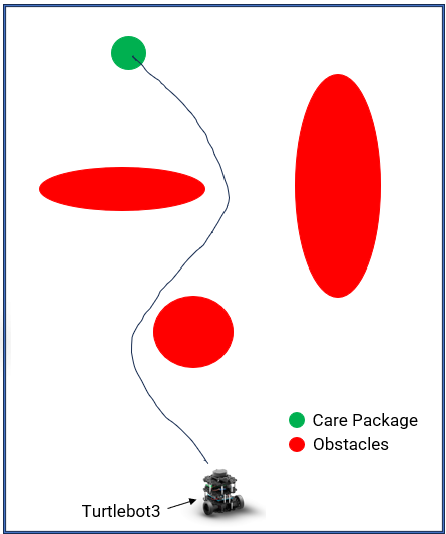
\includegraphics[width=0.4\textwidth]{figs/objective_fig.png} % Scaled to 50% of the text width
    \caption{Mobile Robot Objective}
    \label{fig:proj_obj}
\end{figure}

\paragraph{Dataset} Datasets are collected by the Turtlebot's sensors:
\begin{itemize}
    \item LiDAR (LDS-02 \cite{lds02})
    \begin{itemize}
        \item Angular speed
        \item Measurement angle
        \item 12 point measurements for distance to objects with confidence
    \end{itemize}
    \newpage
    \item Camera (Raspberry Pi Camera \cite{camera})
    \begin{itemize}
        \item Images
        \item Video
    \end{itemize}
    \item Wheel Encoder (XL430-W250 \cite{encoders})
    \begin{itemize}
        \item Positioning
        \item Velocity
        \item Acceleration
        \item Load (torque)
        \item Goal position
    \end{itemize}

\end{itemize}

\section{Problem Definition} \label{sec:problem definition}
For robots to make decisions in stochastic environments, the aforementioned operations require methods for understanding the random variables and conditions presented to them. In the case of this project, for perception/object detection, a target objective needs to be identified. For path planning, optimized pathing needs to be determined based on the mapped environment \cite{lidar_path_planning}. System control should be intelligent such that the mobile robot can compensate for actuator disturbances and sensed error \cite{control_CNN}. The solution to these stochastic problems is a fusion of ML algorithms as discussed thoroughly in Section \ref{sec:methods}. 
% With these solutions, autonomous vehicles can detect an objective with environmental noise and constraints, plan an intelligent path, and control the vehicle without need for dynamic system knowledge.

\section{Methods} \label{sec:methods}
\subsection{Data Pre-Processing}
Filtering and cleaning sensor data is an important step in the ML process and will be performed on sensor data with the following methods:
% LiDAR data can be noisy, and it is important to remove any erroneous or unnecessary points from the point cloud to improve the accuracy of the final product. This can be done using a variety of methods, such as \textbf{density-based filtering or statistical outlier removal}.
\begin{itemize}

\item \textbf{Density-based filtering} (DBSCAN clustering): Density-based clustering non-parametric algorithm: given a set of points in some space, group together points that are closely packed (points with many nearby neighbors), and mark outlier points that lie alone in low-density regions (those whose nearest neighbors are too far away) \cite{scikit-learn-dbscan}.

\item \textbf{Kalman Filtering}: Kalman filtering is utilized to estimate system states given noisy data. Assuming a Gaussian distribution of sensor data, the Kalman filter quickly computes estimated states in the presence of noise using sensor measurements and predicted states \cite{KalmanFilter1D}.
% \item \textbf{Point-cloud outlier removal}:
% \begin{itemize}
% \item \textit{Statistical outlier removal}: removes points that are further away from their neighbors compared to the average for the point cloud

% \item \textit{Radial outlier removal}: removes points that have few neighbors in a given sphere around them

% https://www.open3d.org/docs/0.12.0/tutorial/geometry/pointcloud\_outlier\_removal.html\\

% \end{itemize}
\end{itemize}
\subsection{ML Algorithms}
The robot's mission can be split into three successive tasks, each one associated to a specific algorithm:
\begin{itemize}
    \item Object detection: Finding the objective
    \begin{itemize}
        \item \textit{Model}: Supervised learning - YOLO algorithm \cite{yolo}
        \item \textit{Sensor}: Camera
    \end{itemize}
    \item Mapping: Understanding the environment
    \begin{itemize}
        \item \textit{Model}: Unsupervised learning - CNN for Simultaneous Localization and Mapping \cite{SLAM}
        \item \textit{Sensors}: LiDAR and camera
    \end{itemize}
    \item Control: Determining control commands
    \begin{itemize}
        \item \textit{Model}: Reinforcement Learning - PPO model combined with A* path finding algorithm \cite{PPO_algo}
        \item \textit{Sensors}: Encoders
    \end{itemize}
\end{itemize}

\section{Results and Discussion} \label{sec:results}
The goal of this project is to autonomously navigate a mobile robot to an objective, with the following scoring and expected results. Team Gantt chart (Figure \ref{fig:gantt}) and contribution table (Table \ref{tab:contributions}) are shown below.\\
\begin{itemize}
\item \textbf{Scoring}:
\begin{itemize}
\item Jaccard score for YOLO, with a goal of 0.9+
\item Silhouette clustering, with a goal of 0.7+
\item Minimize Cross-Entropy Loss for reinforcement learning, with a goal of $<10\%$ error
\end{itemize}
\item \textbf{Expected Results}:
\begin{itemize}
\item Final position distance from extraction point: Be within 1/3 meter
\item Time requirement: Reach the extraction point within 60 seconds
\end{itemize}
\end{itemize}

\begin{figure}[htp]
    \centering
    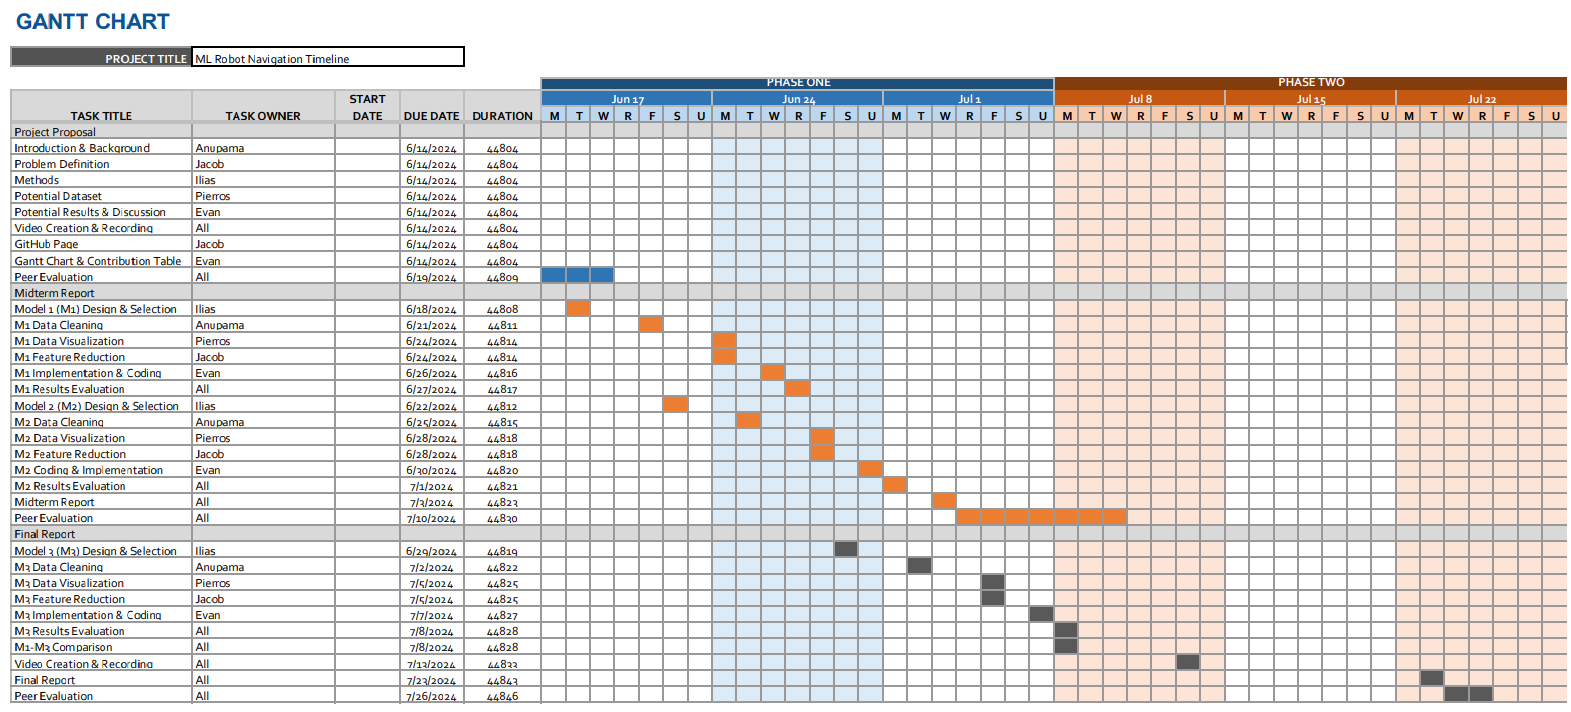
\includegraphics[width=1.0\textwidth]{figs/gantt.png} % Scaled to 50% of the text width
    \caption{Team Gantt Chart}
    \label{fig:gantt}
\end{figure}

\begin{table}[ht]
    \centering
        \caption{Team Contributions}
    \label{tab:contributions}
    \begin{tabular}{|l|p{10cm}|}
        \hline
        \textbf{Name} & \textbf{Proposal Contributions} \\
        \hline
        Jacob Blevins & Literature review, problem definition, and initial robot testing \\
        \hline
        Evan Boekweg & Metrics, goals, and results \\
        \hline
        Ilias Baali & ML algorithms and models \\
        \hline
        Anupama Nair & Data pre-processing \\
        \hline
        Pierros-Christos Skafidas & Dataset review \\
        \hline
    \end{tabular}
\end{table}
\newpage

\bibliographystyle{asmejour}   %% .bst file that follows ASME journal format. Do not change.
\bibliography{sample}


\end{document}
